\documentclass[10pt,notitlepage,nofootinbib,preprintnumbers,showpacs]{revtex4-2}
\usepackage{color,graphicx,epsfig}
\usepackage{amsmath}
\usepackage{amssymb}
\usepackage[utf8]{inputenc}
\usepackage[usenames,dvipsnames]{xcolor}
\usepackage{tikz}
\usepackage{tikz-feynman}
\usetikzlibrary{calc,patterns,angles,quotes,arrows}

\begin{document}

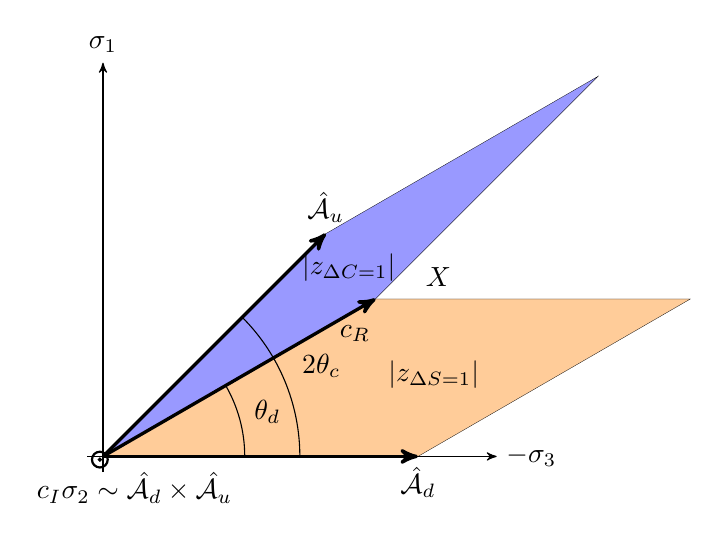
\begin{tikzpicture}[
			scale=2,
			axis/.style={thin, ->, >=stealth'},
			important line/.style={very thick, ->, >=stealth'},
			every node/.style={color=black, opacity=1.}
			]
			%points
			\coordinate (origin) at (0.,0.);
			\coordinate (poly1) at (1.73, 1.0);
			\coordinate (poly2) at (3.73, 1.0);
			\coordinate (poly3) at (2., 0.0); 
			\coordinate (poly4) at (1.4142, 1.4142);
			\coordinate (poly5) at (3.1442, 2.4142); 
			\coordinate (poly6) at (1.73, 1.0); 
			\coordinate (origo) at (0.25,0.);
			\coordinate (pivot1) at (10.,5.8);
			\coordinate (pivot2) at (10.,0);
                        \coordinate (pivot3) at (10.,10);
			%Fills
			\draw[black, ultra thin, fill=orange, fill opacity=0.4] (0.,0.) -- (1.73, 1.0) -- (3.73, 1.0) -- (2., 0.0) -- cycle;
			\draw[black, ultra thin, fill=blue, fill opacity=0.4] (0.,0.) --(1.4142, 1.4142) -- (3.1442, 2.4142) -- (1.73, 1.0) -- cycle;
                        % axes
                        \draw[axis] (-0.1,0)  -- (2.5,0) node(xline)[right]
                        {$- \sigma_3$};
                        \draw[axis] (0,-0.1) -- (0,2.5) node(yline)[above] {$\sigma_1$};
			% Lines                     
			\draw[important line] (0,0.) -- (1.4142, 1.4142) node(zline)[above] {$\hat{\mathcal{A}}_u$};
			\draw[important line] (0,0.) -- (2., 0.0) node(zline)[below] {$\hat{\mathcal{A}}_d$};
			\draw[important line] (0,0.) -- (1.73, 1.0) node(zline)[above right] {};
			\pic [draw, -, angle radius=18mm, angle eccentricity=1.2, "$\theta_d$"] {angle = pivot2--origin--pivot1};
                        \pic [draw, -, angle radius=25mm, angle eccentricity=1.2, "$2\theta_c$"] {angle = pivot2--origin--pivot3};
			%Nodes
			\node (none) at (1.56,1.2) {$|z_{\Delta C = 1}|$};
			\node (none) at (2.1,0.52) {$|z_{\Delta S = 1}|$};
			\node (none) at (2.13,1.14) {$X$};
                        \node (none) at (1.6,0.78) {$c_R$};
                        \draw [thick] (-0.02,-0.02) circle [radius=0.05];
                        \draw [fill] (-0.02,-0.02) circle [radius=0.01];
                        \node (none) at (0.2,-0.2) {$c_I \sigma_2 \sim \hat{\mathcal{A}_d} \times \hat{\mathcal{A}_u}$};
                      \end{tikzpicture}

\end{document}